\documentclass[12pt, a4paper]{article}
\usepackage[left=3cm, right = 2cm, vmargin=2cm]{geometry}
\usepackage{microtype}
\usepackage{graphicx}
\usepackage{hyperref}
\usepackage[english]{babel}
\usepackage{setspace}
\usepackage{xcolor}
\usepackage{multicol}
\usepackage{float}
\usepackage{amsmath}
\usepackage{amssymb}
\usepackage{mathtools}
\usepackage{titlesec}
\usepackage{bbm}
\usepackage{booktabs}
\usepackage[font=small,skip=2pt]{caption}
\usepackage[
backend=biber,
style=authoryear,
]{biblatex}
\usepackage{amsthm}% http://ctan.org/pkg/amsthm

\DeclarePairedDelimiter\ceil{\lceil}{\rceil}
\DeclarePairedDelimiter\floor{\lfloor}{\rfloor}

\newtheoremstyle{MAstyle}
{\topsep} % Space above
{\topsep} % Space below
{} % Body font
{} % Indent amount
{\bfseries} % Theorem head font
{\newline} % Punctuation after theorem head
{.5em} % Space after theorem head
{} % Theorem head spec (can be left empty, meaning `normal')

\theoremstyle{MAstyle} \newtheorem{assumption}{Assumption}[section]
\theoremstyle{MAstyle} \newtheorem{definition}{Definition}[section]
\theoremstyle{MAstyle} \newtheorem{theorem}{Theorem}[section]

\titleformat*{\section}{\Large\bfseries}
\titleformat*{\subsection}{\large\bfseries}

\addbibresource{thesis_bibliography.bib}
\onehalfspacing
\parindent=0pt

\begin{document}
	
	\title{{\huge Bugni and Horowitz (2021) Permutation Tests\\ for the Equality of Distributions of\\ Functional Data}}
	\date{}
	\maketitle
	\thispagestyle{empty}
	\vspace{1.5 cm}
	\begin{center}
		
		\Large
		Master's Thesis presented to the\\
		Department of Economics at the\\
		Rheinische Friedrich-Wilhelms-Universität Bonn
		\vspace{1.5cm}

		\large
		In Partial Fulfillment of the Requirements for the Degree of\\
		Master of Science (M.Sc.)
		
		\vspace{3cm}
		
		Supervisor: Prof. Dr. Dominik Liebl
		
		\vspace{3cm}
		
		Submitted in June 2022 by: \\
		Jakob R. Juergens\\
		Matriculation Number: 2996491
	\end{center}
	
	\newpage
	
	\thispagestyle{empty}
	\tableofcontents
	\thispagestyle{empty}
	
	\newpage
	\pagenumbering{arabic}
	
	\section{Introduction}
		In modern economics, it is becoming more and more common to use data measured at a very high frequency. As the frequency of observing a variable increases, it often becomes more natural to view the data not as a sequence of distinct observation points but as a smooth curve that describes the variable over time.
		This idea, to think of observations as measurements of a continuous process, is the motivating thought behind functional data analysis. Functional data analysis is a branch of statistics that has its beginnings in the 1940s and 1950s in the works of Ulf Grenander and Kari Karhunen. It gained traction during the following decades and focused more on possible applications during the 1990s. In economics, functional data analysis is still a relatively exotic field, but it is beginning to become more established, which can be seen in the works of, for example, {\color{red} hier Autoren einfuegen}.\\
		
		A typical question in economics is whether observations from two or more data sets, e.g., data generated by treatment and control groups, are systematically different across groups. In statistical terms, this can be formulated as whether the same stochastic process generated observations in both data sets.				
		This question can also occur in functional data analysis, where each observation in a data set is itself a smooth curve. \cite{bugni_permutation_2021} develop a permutation test that tries to answer this question by combining two test statistics. To explore their approach, it is first necessary to introduce some theoretical concepts.
		Section \ref{FDA} introduces the necessary concepts from functional data analysis. 
		Section \ref{CvM_Tests} explores the theory around Cram\'{e}r-von Mises tests and section \ref{Permutation_Tests} introduces the necessary background in Permutation Testing.
		After explaining these concepts, section \ref{Bugni_Horowitz_2021} focuses on the test developed in \cite{bugni_permutation_2021} for the case of a two-sample test. Section \ref{closed_testing} introduces the concept of closed testing procedures, which is used in Section \ref{frequency_identification} to develop an extension to the original test, that could be used to identify specific types of violations of the nullhypothesis. Section \ref{Simulation_Study} replicates the results from the simulation study in the paper and expands on certain aspects. Section \ref{Application} explores their usefulness in an application to half-hourly electricity demand data from Adelaide.
		Finally, Section \ref{Outlook} gives an Outlook on possible extensions of the underlying idea and addresses some problems and shortcomings of the presented results.
	
	\section{Functional Data Analysis}\label{FDA}
		The overarching concept of functional data analysis is to incorporate observations that are functional in nature. In this context, a functional observation can often be understood as a smooth curve. A classical example of this is shown in Figure \ref{growth_curves}. It presents data provided in the R package \textit{fda}\footcite{fda} and shows growth curves of 93 humans up to the age of 18.
		\begin{figure}[H]
			\makebox[\textwidth][c]{
			\includegraphics[width = 1.1\textwidth]{../Graphics/growth\_curves.PDF}
		}
			\caption{Human Growth Curves up to the Age of 18}
			\label{growth_curves}
		\end{figure}
		Even though the measurements were taken at discrete ages, it is clear that each human has a height at every point in time. The data points are only measurements of this continuous curve. The higher the measurement frequency, the closer we get to data that resembles the curve itself.
		In many cases functional data analysis restricts its scope to subsets of the functions $f:\mathbb{R} \rightarrow \mathbb{R}$.
		As these are inherently infinite-dimensional, it is necessary to introduce additional theory to appropriately deal with their unique properties. Sections \ref{Square_Integrable_Functions} and \ref{bases_L2} closely follow \cite{hsing_theoretical_2015} who provide a detailed introduction into the theory of functional data analysis.
		
		\begin{itemize}
			\item \cite{ramsay_functional_2005}
			\item \cite{kokoszka_introduction_2021}
		\end{itemize}
	
		\subsection{Hilbert Space of Square Integrable Functions}\label{Square_Integrable_Functions}
			\begin{definition}[Inner Product]
				A function $\langle \cdot , \cdot \rangle : \mathbb{V}^2 \rightarrow \mathbb{F}$ on a vector space $\mathbb{V}$ over a field $\mathbb{F}$ is called an inner product if the following four conditions hold for all $v, v_1, v_2 \in \mathbb{V}$ and $a_1, a_2 \in \mathbb{F}$.
				\begin{multicols}{2}
					\begin{enumerate}
						\item $\langle v,v \rangle \geq 0$
						\item $\langle v,v \rangle = 0$ if $v = 0$
						\item $\langle a_1 v_1 + a_2 v_2, v \rangle = a_1 \langle v_1, v \rangle + a_2 \langle v_2, v \rangle$
						\item $\langle v_1, v_2 \rangle = \overline{\langle v_2, v_1 \rangle}$
					\end{enumerate}
				\end{multicols}
			\end{definition}
			As this thesis is limited to the case $\mathbb{F} = \mathbb{R}$, property 4 can be restated as $\langle v_1, v_2 \rangle = \langle v_2, v_1 \rangle$, as the complex conjugate of a real number is the number itself. Similar to the case of Euclidean space, we say that two elements $v_1$ and $v_2$ of the inner product space are orthogonal if $\langle v_1, v_2 \rangle = 0$.
			
			\begin{definition}[Inner Product Spaces and Hilbert Spaces]
				A vector space with an associated inner product is called an inner product space.
				An inner product space that is complete with respect to the distance induced by the norm $\| v \| = \sqrt{\langle v, v\rangle}$ is called a Hilbert space.
			\end{definition}
			Hilbert spaces play an important role in functional data analysis and many methods such as for example functional linear regression make extensive use of their properties. In the context of this thesis, the idea of Hilbert spaces is necessary to adequately describe objects such as random functions or probability measures on Hilbert spaces that are used extensively in \cite{bugni_permutation_2021}.\\
			
			Analogously to the case of a vector space, it is useful to express elements of a Hilbert space as linear combinations of a set of elements. However, as elements of Hilbert spaces can be potentially infinite dimensional, the classical idea of a finite basis that can be used to express every element has to be extended.
		
			\begin{definition}[Closed Span]
				The closed span of a subset $A$ of some normed space, e.g. a normed vector space or a Hilbert space, is the closure of $\textit{span}\left(A\right)$ with respect to the distance induced by the norm of the space. In the following it is denoted by $\overline{{\textit{span}\left(A\right)}}$.
			\end{definition}
		
			{\color{red} This is verbatim!}
			\begin{definition}[Orthonormal Sequence in a Hilbert Space]
				Let $\{x_n\}$ be a countable collection of elements in a Hilbert space such that every finite subcollection of $\{x_n\}$ is linearly independent. Define $e_1 = \frac{x_1}{\| x_1 \|}$ and $e_i = \frac{v_i}{\| v_i \|}$ for 
				$$v_i = x_i - \sum_{j = 1}^{i - 1}\langle x_i, e_j\rangle e_j.$$
				Then, $\{e_n\}$ is an orthonormal sequence and $\overline{{\textit{span}\left(\{x_n\}\right)}} = \overline{{\textit{span}\left(\{e_n\}\right)}}$
			\end{definition}
		
			The definition of the closed span and orthonormal sequences makes it possible to define the analogon of the basis in finite dimensional vector spaces for the case of potentially infinite-dimensional Hilbert spaces.
		
			{\color{red} This is verbatim!}
			\begin{definition}[Orthonormal Basis of a Hilbert Space]
				An orthonormal sequence $\{e_n\}$ in a Hilbert space $\mathbb{H}$ is called an orthonormal basis of $\mathbb{H}$ if $\overline{{\textit{span}\left(\{e_n\}\right)}} = \mathbb{H}$. Bases like this are typically called Schauder bases to differentiate them from Hamel bases which are often used in the study of vector spaces. The difference between these is that a Schauder basis can represent elements of the corresponding space as infinite sums of its elements, whereas a Hamel basis can only use finite linear combinations.
			\end{definition}
			
			A special class of Hilbert spaces that is used in most contexts that are relevant in functional data analysis are so called separable Hilbert spaces. Their properties will allow significant simplifications in the calculation of specific test statistics that are at the core of \cite{bugni_permutation_2021}.
			\begin{definition}[Separable Hilbert Space]
				A Hilbert space that possesses a countable complete orthonormal basis is called separable Hilbert space.
			\end{definition}
			Using the axiom of choice, it is possible to show that every Hilbert space possesses an orthonormal basis, which will be used in the derivation of an asymptotic distribution for a test statistic later in this thesis.\\
			
			The Hilbert space that is most important in functional data analysis is the space of square integrable functions. However, this leads to the case that often square integrability is assumed by default and it is interesting to consider whether this property is actually necessary.		
			\begin{definition}[Hilbert Space of Square Integrable Functions]
				
				The space of square integrable functions on a closed interval $\mathcal{I}$ together with the norm $\langle f,g\rangle = \int_{\mathcal{I}} f(t)g(t) \mathrm{d}t$ is a Hilbert space.
				A function $f: \mathcal{I} \rightarrow \mathbb{R}$ is called square-integrable if the following condition holds.
				\begin{equation}
					\int_{A} \left[f(t)\right]^2\mathrm{d}t < \infty
				\end{equation}
				To give the space the properties that are typically desired in Functional data analysis, it is typically defined as a space of equivalence classes, where to functions are seen as equivalent if they differ at most on a set of Lebesgue-measure zero. The Hilbert space of all square integrable functions on $\mathcal{I}$ is denoted by $\mathbb{L}_2(\mathcal{I})$.
			\end{definition}
			
			In most cases, $A$ is chosen as a closed interval of $\mathbb{R}$. Without loss of generality, we can reduce our treatment to the case of $\mathcal{I} = [0,1]$.
			
			\subsection{$\mathbb{L}_2(\mathcal{I})$ as defined in \cite{bugni_permutation_2021}}
			Deviating from the norm in functional data analysis, \cite{bugni_permutation_2021} define two square-integrable functions to be distinct even if they differ only on a set of Lebesgue-measure zero. To distinguish between the typical case presented in the previous section, let $\mathbb{L}_2(\mathcal{I})$ denote the Hilbert space of square-integrable functions and $\mathbb{L}^{*}_2(\mathcal{I})$ the square-integrable functions under the the convention from \cite{bugni_permutation_2021}.\\
			
			Using $\mathbb{L}^{*}_2(\mathcal{I})$ creates some interesting theoretical challenges, as the resulting object is in fact not a Hilbert space. To understand the theoretical problems that can occur, I first introduce some additional concepts to illustrate the challenges.
			\begin{definition}[Norm and Seminorm]
				A function $p : \mathbb{V} \rightarrow \mathbb{F}$ on a vector space $\mathbb{V}$ over a field $\mathbb{F}$ is called a norm if the following four conditions hold for all $v,u \in \mathbb{V}$ and $s \in \mathbb{F}$.
				\begin{multicols}{2}
					\begin{enumerate}
						\item $p(v + u) \leq p(v) + p(u)$
						\item $p(sv) = |s| p(v)$
						\item $p(v) \geq 0$
						\item $p(v) = 0 \implies v = 0$
					\end{enumerate}
				\end{multicols}
				If $p : \mathbb{V} \rightarrow \mathbb{F}$ fulfills only properties (1) to (3) it is called a seminorm.
			\end{definition}
			
			In the same way a norm induces a distance on its corresponding normed vectorspace, a seminorm $p$ induces a so-called pseudometric $d$. It is given by $d(v,u) = p(u-v)$.
			
			{\color{red} This is from Wikipedia!!!}
			\begin{definition}[Pseudometric Space]
				A pseudometric space $\left(X, d\right)$ is a set $X$ together with a function $d:X\times X \rightarrow \mathbb{R}_{\geq 0}$, such that $\forall x,y,z \in X$ the following properties hold.
				\begin{multicols}{2}
					\begin{enumerate}
						\item $d(x,x) = 0$
						\item $d(x,y) = d(y,x)$
						\item $d(x,z) \leq d(x,y) + d(y,z)$
					\end{enumerate}
				\end{multicols}
				Therefore, deviating from a metric space, two distinct points in a pseudometric space can have a distance of zero $d(x,y) = 0$ for $x \neq y$.
			\end{definition}
			
			That $\mathbb{L}^{*}_2(\mathcal{I})$ is not a Hilbert space becomes clear, when checking the for the properties of the norm induced by the inner product $\| v \| = \sqrt{\langle v, v\rangle}$.
			One of the properties that has to be fulfilled by a norm is $\| v \| = 0 \Longleftrightarrow v = 0$.			
			Let $f:[0,1] \rightarrow \mathbb{R}$ be given by $f(x) = \mathbbm{1}\left[x = 0.5\right]$. Then we can evaluate the following expression to create a contradiction to the norm properties.
			\begin{equation}
				\| f \| = \sqrt{\langle f, f\rangle} = \sqrt{\int_{0}^{1} \left[f(t)\right]^2\mathrm{d}t } = 0
			\end{equation}
			As $f$ is not the zero element of this space, this is a violation of positive definiteness. Positive definiteness applied to the case at hand, states that $\forall v \in \mathbb{L}_2\left(\mathcal{I}\right) \| v \| = 0 \implies v(x) = 0 \quad \forall x \in \mathcal{I}$  $\forall v \in $. Instead, $\| v \| = \sqrt{\langle v, v\rangle}$ is a seminorm and the defined space should more correctly be treated as a pseudometric space.\\
			
			{\color{red} This is from Wikipedia!!!}
			\begin{definition}[Hausdorff Space]
				A Hausdorff space is a topological space where for any two distinct points $x$ and $y$, there exist a neighborhood $U$ of $x$ and a nieghborhood $V$ of $y$ such that $U$ and $V$ are disjoint. This property is also called neighborhood-separability.
			\end{definition}
			
			One problem of $\mathbb{L}^{*}_2(\mathcal{I})$ is, that if we give the space the topology induced by the obvious seminorm, the resulting space would not be Hausdorff. Thus, limits in the later part of \cite{bugni_permutation_2021} would not be defined.
			A second problem is, that it is not clear how a Schauder basis would be defined for a pseudometric space such as $\mathbb{L}^{*}_2(\mathcal{I})$ and that typical existence results for orthonormal bases might not be available.\\			
			
			In the following, I will therefore restrict my analysis to {\color{red} Hier weiterschreiben!}

			
			
		\subsection{Bases of $\mathbb{L}_2$}\label{bases_L2}
			
			One commonly used orthonormal basis of $\mathbb{L}^2([0,1])$ is the Fourier Basis. It consists of a series of functions $\left(\phi_{i}^{F}(x)\right)_{i \in \mathbb{N}}$ taken from the terms of the sine-cosine form of the Fourier series.
			\begin{equation}
				\phi_{i}^{F}(x) = 
				\begin{cases}
					1 & \text{if} \quad i = 1\\
					\sqrt{2} \cos(\pi i x) & \text{if} \quad i \quad \text{is even} \\
					\sqrt{2} \sin(\pi (i-1)x) & \text{otherwise}
				\end{cases}
			\end{equation}
			Figure \ref{fourier_basis} shows the first seven Fourier basis functions on $[0,1]$.
			\begin{figure}[H]
				\includegraphics[width = \textwidth]{../Graphics/fourier\_basis.PDF}
				\caption{The first seven Fourier basis functions}
				\label{fourier_basis}
			\end{figure}
			A proof that the Fourier basis is in fact an orthonormal basis of $\mathbb{L}^2([0,1])$ can be found in section 2.4 of \cite{hsing_theoretical_2015}. As the Fourier basis is a countable orthonormal basis of $\mathbb{L}^2([0,1])$, we can follow that $\mathbb{L}^2([0,1])$ is a separable Hilbert space, which will be useful in further parts of this thesis.
	
		\subsection{Random Functions}
			Random functions are a special case of general random variables. To understand their connection to the general concepts it is therefore useful to remind ourselves of the definition of a random variable. Paraphrasing from \cite{bauer_probability_2011} this can take the following form.
			\begin{definition}[Random Variable]
				Let $\left(\Omega, \mathcal{A}, \mathcal{P}\right)$ be a probability space and $\left(\Omega', \mathcal{A}'\right)$ be a measure space. Then every $\mathcal{A}$-$\mathcal{A}'$-measurable function $X:\Omega \rightarrow \Omega'$ is called a $\left(\Omega', \mathcal{A}'\right)$-random variable.
			\end{definition}
		
			\begin{definition}[Random Function]
				A random variable that realizes in a function space, e.g. $\mathbb{L}^2[0,1]$, is called a random function.
			\end{definition}
		
		\subsection{Probability Measures on $\mathbb{L}_2$}\label{prob_measures_l2}
			In later parts of this thesis, it will be important to evaluate expectations of a functional on $\mathbb{L}_2$. For this to make sense, it is necessary to explore how we can define probability measures on function spaces. Additionally, it is interesting to take a look at some special properties of the probability measures used in \cite{bugni_permutation_2021} as these allow for significant simplifications in the evaluation of terms in later parts of the paper. As the formal treatment of these aspects would be mathematically very involved, this section shall serve to give intuition. \cite{gihman_theory_2004} and \cite{skorohod_integration_1974} give a rigorous treatment of all the necessary theory.
			
			\begin{theorem}[Kolmogorov Extension Theorem]
				content
			\end{theorem}
		
			\subsubsection{Probability Measures induced by Random Functions}
				If instead we assume an existing random function $Z(t)$, it is useful ... {\color{red} Hier weiterschreiben}
		
		\subsection{Functional Integration on $\mathbb{L}_2$}
			\begin{itemize}
				\item Perturbation theory
			\end{itemize}
		
			In one of the test statistics used in \cite{bugni_permutation_2021}, it is necessary to integrate over a function space. Therefore, it is necessary to explore the ideas of functional integration and integration on Hilbert spaces more general. Because of the special case relevant to the test statistic, integration on separable Hilbert spaces shall take a special focus.
			\begin{equation}
				\int_{\mathbb{L}_2(\mathcal{I})} G\left[f\right] \left[Df\right] = \int_{-\infty}^{\infty}\dots\int_{-\infty}^{\infty} G\left[f\right] \prod_{x} \mathrm{d}f(x)
			\end{equation}
		
			If a representation in terms of an orthogonal functional basis is possible:
			\begin{equation}
				\int_{\mathbb{L}_2(\mathcal{I})} G\left[f\right] \left[Df\right] = \int_{-\infty}^{\infty}\dots\int_{-\infty}^{\infty} G\left(f_1, f_2, \dots\right) \prod_{n} \mathrm{d}f_n
			\end{equation}
		
			An in-depth treatment of integration on Hilbert spaces is available in \cite{skorohod_integration_1974}.
		
	\section{Cram\'{e}r-von Mises Tests}\label{CvM_Tests}
		In applied econometrics, it is often interesting to ask whether the same stochastic process generated the observations in two distinct data sets. In an experimental setting, we could ask whether a treatment assigned at random to a subset of agents changed the distribution of an outcome variable. 
		One approach to answering this question is given by the two-sample Cram\'{e}r-von Mises test.
		
		\begin{itemize}
			\item \cite{darling_kolmogorov-smirnov_1957}
			\item \cite{anderson_asymptotic_1952}
			\item \cite{buning_nichtparametrische_2013}
		\end{itemize}
	
		\subsection{Empirical Distribution Functions}
			
			\cite{gibbons_nonparametric_2021}
			\begin{definition}[Order Statistic]\label{Order_Stat}
				
				Let $\{x_i \: \vert \: i = 1, \dots , n\}$ be a random sample from a population with continuous cumulative distribution function $F_X$. Then there almost surely exists a unique ordered arrangement within the sample. 
				
				$$X_{(1)} < X_{(2)} < \dots < X_{(n)}$$
				
				$X_{(r)} \quad r \in \{1, \dots, n\}$ is called the $r$th-order statistic.	
			\end{definition}
		
			\begin{definition}[Empirical Distribution Function]
				\begin{equation}
					F_{n}(x) = \begin{cases}
						0 & \quad \text{if} \quad  x < x_{(1)} \\
						\frac{r}{n} & \quad \text{if} \quad  x_{(r)} \leq x < x_{(r + 1)} \\
						1 & \quad \text{if} \quad  x \geq x_{(n)}
					\end{cases}
				\end{equation}
			\end{definition}
		
		\subsection{Assumptions}
		
		\subsection{Nullhypothesis}
			Let $\{x_1, \dots , x_n\}$ and $\{y_1, \dots , y_m\}$ be two data sets generated by random variables $X \sim_{\text{i.i.d.}} F(t)$ and $Y \sim_{\text{i.i.d.}} G(t)$.
			Then, we can formulate the Nullhypothesis that both samples were independently generated by random variables following the same distribution function.
			\begin{equation}
				\begin{split}
					H_0&: F(t) = G(t) \quad \forall t \in \mathbb{R}\\
					H_1&: \exists t \in \mathbb{R} \quad \text{s.t.} \quad F(t) \neq G(t)
				\end{split}
			\end{equation}
			
		\subsection{Two-Sample Cram\'{e}r-von Mises Statistic}
			
			\cite{buning_nichtparametrische_2013}
			\begin{equation}
				C_{m,n} = \left(\frac{nm}{n+m}\right) \int_{-\infty}^{\infty}\left(F_{m}(x) - G_{n}(x)\right)^{2} \mathrm{d} \left(\frac{m F_{m}(x) + n G_{n}(x)}{m+n}\right)
			\end{equation}
			\cite{anderson_distribution_1962} explores the small sample distribution of this test statistic and provides a comparison to the limiting distribution derived by \cite{rosenblatt_limit_1952} and \cite{fisz_result_1960}.
		
		\subsection{Asymptotic Distribution}
			As shown by the previously mentioned authors, under the Nullhypothesis that both samples were independently generated by random variables sharing the same distribution function, we can find the following limiting distribution of $C_{m,n}$.
			\begin{equation}
				\begin{split}
					C_{m,n} &\xrightarrow{\text{d}} \int_{0}^{1} \left(Z(u) + \left(1 + \lambda\right)^{-\frac{1}{2}} f(u) - \left[\frac{\lambda}{1+\lambda}\right]^{\frac{1}{2}}g(u)\right)^2 \mathrm{d}u \\
					\text{as} \quad &n \rightarrow \infty, \quad m \rightarrow \infty, \quad \frac{n}{m} \rightarrow \lambda \in \mathbb{R}
				\end{split}
			\end{equation}
			Here, $Z(u)$ is a Gaussian stochastic process with the following properties.
			\begin{itemize}
				\item $\mathbb{E}\left[Z(u)\right] = 0 \quad \forall u \in [0,1]$
				\item $Cov\left(Z(u), Z(v)\right) = \min(u,v) - uv \quad \forall u,v \in [0,1]$
			\end{itemize}					
			
	\section{Permutation Tests}\label{Permutation_Tests}
		In layman's terms, the idea of a permutation test is the following: if two samples show distinctly different properties, that will lead to differences in an appropriately chosen summary statistic. If we were to permute the elements of the groups randomly, we would expect these differences to disappear.
		Permutation tests formalize this intuition. The following section closely follows chapter 15 from \cite{lehmann_testing_2005}.
		
		\begin{itemize}
			\item \cite{van_der_vaart_weak_1996}
		\end{itemize}
	
		\subsection{Functional Principle of Permutation Tests}
		
			One on the defining features of each test is its Nullhypothesis. For the case of randomization tests, we can formulate it quite generally. Let $X$ be data taking values in a sample space $\mathcal{X}$. Then, the hypothesis is that the probability law $P$ generating $X$ belongs to a family of distributions $\Omega_0$. \cite{lehmann_testing_2005} define an assumption called the randomization hypothesis that allows for the construction of randomization tests. As permutation tests are a special case of randomization tests, we can specialize this definition to the case under consideration.
			\begin{assumption}[Randomization Hypothesis]\label{rand_hypo}
				 Let $G$ be a finite group of transformations $g: \mathcal{X} \rightarrow \mathcal{X}$. Under the Nullhypothesis of the randomization test, the distribution of $X$ is invariant under the transformations $g \in G$. In other words, $gX$ and $X$ have the same distribution whenever $X$ has distribution $P \in \Omega_0$.
			\end{assumption}
			Under this assumption one can construct a permutation test based on any test statistic $T:\mathcal{X} \rightarrow \mathbb{R}$ that is suitable to test the Nullhypothesis under consideration. Suppose that $G$ has $M$ elements, then given $X = x$, let 
			$$T_{(1)}(x) \leq T_{(2)}(x) \leq \dots \leq T_{(M)}(x) $$
			be the ordered values of the test statistic $T(gx)$ as described in Definition \ref{Order_Stat} as $g$ varies over $G$. For a fixed nominal level $\alpha \in (0,1)$, define $k = M - \lfloor M\alpha \rfloor$. Additionally define the following two objects.
			\begin{multicols}{2}
				\noindent
				\begin{equation*}
					M^{+} = \sum_{m = 1}^{M}\mathbbm{1}\left[T_{(m)}(x) > T_{(k)}(x)\right]
				\end{equation*}
				\begin{equation}
					M^{0} = \sum_{m = 1}^{M}\mathbbm{1}\left[T_{(m)}(x) = T_{(k)}(x)\right]
				\end{equation}
			\end{multicols}
			
			\begin{definition}[Randomization Test Function]\label{RandTestFunc}
				We define the Randomization Test Function as the following function $\phi: \mathcal{X} \rightarrow \mathbb{R}$.
					\begin{equation*}
						\phi(x) = \begin{cases}
							1 &\text{if} \ T > T_{(k)}(x) \\
							a &\text{if} \ T = T_{(k)}(x) \\
							0 &\text{if} \ T < T_{(k)}(x) \\
						\end{cases} \quad \text{where} \quad
						a = \frac{M\alpha - M^{+}(x)}{M^{0}(x)}
					\end{equation*}
				
			\end{definition}
			Under Assumption \ref{rand_hypo}, it is possible to show that, given a test statistic $T = T(X)$, the resulting test $\phi$ has size $\alpha$.
			\begin{equation}
				\mathbb{E}_{P}\left[\phi(X)\right] = \alpha \quad \forall P \in \Omega_0
			\end{equation}
			
		
			\cite{lehmann_testing_2005} explore the example of testing for the equality of the generating probability laws of two independent samples. This is precisely the relevant application for the permutation variant of the two-sample Cram\'{e}r-von Mises test that \cite{bugni_permutation_2021} extend to the setting of functional data. \\
			
			\begin{definition}[Permutation]
				Let $S$ be a set, then a permutation of $S$ is a bijective function $\pi: S \rightarrow S$.
			\end{definition}
			If $S$ is a finite set with $N$ elements, there are $N!$ different permutations. If we apply this idea to the setting of two samples with $n$ and $m$ observations respectively, there are $(n+m)!$ permutations in the combined set of observations. One way of describing the corresponding group of transformations $G$ is shown in Equation \ref{Permutations}.
			\begin{equation}\label{Permutations}
				\begin{split}
					\Pi_N &= \left\{\pi: \left\{1, \dots, N \right\} \rightarrow \left\{1, \dots, N \right\} \ \vert \ \pi \ \text{is bijective} \right\} \\
					G &= \left\{g:\mathbb{R}^N \rightarrow \mathbb{R}^N \ \vert \ \exists \pi \in \Pi_N \ \forall x \in \mathbb{R}^N \ g(x) = \left(x_{\pi(1)}, \dots, x_{\pi(N)}\right) \right\}
				\end{split}
			\end{equation}
			
		 
			Number of Combinations: $\binom{m+n}{m}$\\
			
			For my implementation, I chose the latter variant.
	
		\subsection{Size and Power}
		
	\section{Test by Bugni and Horowitz (2021)}\label{Bugni_Horowitz_2021}
	
		In \cite{bugni_permutation_2021}, the authors devise a permutation test for the equality of the distribution of two samples of functional data. To define the exact hypothesis, it is therefore necessary to define a distribution function for a random variable realizing in $\mathbb{L}_2(\mathcal{I})$.
		\begin{definition}[Distribution Function of a Random Function]
			Let $X:\Omega \rightarrow \mathbb{L}_2(\mathcal{I})$ be a random function realizing in the square-integrable functions. Then its distribution function is defined as the following object.
			\begin{equation*}
				F_X(z) = \mathbb{P}\left[X(t) \leq z(t) \quad \forall t \in \mathcal{I}\right] \quad z \in \mathbb{L}_2(\mathcal{I})
			\end{equation*}
		\end{definition}
		Deviating from the norm in functional data analysis, the authors assume that two functions $z_1, z_2 \in \mathbb{L}_2(\mathcal{I})$ are distinct even if they only differ on a set of Lebesgue-measure zero.\footnote{Does this create a problem about the Fourier basis being a complete orthonormal basis of the space?}
		
		\subsection{Assumptions}
		
			\begin{assumption} Contains two assumptions
				\begin{enumerate}
					\item $X(t)$ and $Y(t)$ are separable, $\mu$-measurable stochastic processes.
					\item $\{X_i(t) \: \vert \: i = 1, \dots, n\}$ is an independent random sample of the process $X(t)$. \\
					$\{Y_i(t) \: \vert \: i = 1, \dots, m\}$ is an independent random sample of $Y(t)$ and is independent of $\{X_i(t) \: \vert \: i = 1, \dots, n\}$.
				\end{enumerate}
			\end{assumption}
		
			\begin{definition}[Separable Stochastic Process]
				{\color{red} From Wikipedia:} A real-valued continuous time stochastic process $X$ with a probability space $\left(\Omega, \mathcal{F}, \mathcal{P}\right)$ is separable if its index set $T$ has a dense countable subset $U \subset T$ and there is a set $\Omega_0 \subset \Omega$ of probability zero, so $\mathcal{P}\left(\Omega_0\right) = 0$, such that for every open set $G \subset T$ and every closed set $F \subset \mathbb{R}$ the two events $\left\{X_t \in F \quad \forall t \in G \cap U\right\}$ and $\left\{X_t \in F \quad \forall t \in G\right\}$ differ from each other at most on a subset $\Omega_0$.
			\end{definition}
		
			In less theoretical terms this means that the process is determined by its values on a countable subset of points of its index set.
		
			\begin{assumption}
				$\mathbb{E}X(t)$ and $\mathbb{E}Y(t)$ exist and are finite for all $t \in [0, T]$.
			\end{assumption}
		
			\begin{assumption}\label{continuous_observation}
				$X_i(t)$ and $Y_i(t)$ are observed for all $t \in \mathcal{I}$.
			\end{assumption}
			Assumption \ref{continuous_observation} can be relaxed and a similar test can be constructed for the case of discretely observed processes. This variation of the test will not be addressed in this thesis. However, \cite{bugni_permutation_2021} provide a description of how to extend their idea to this common scenario.
	
		\subsection{Nullhypothesis}
			As with most permutation tests, the null hypothesis of the test presented by \cite{bugni_permutation_2021} is distributional in nature and is formulated by the authors as follows.
			\begin{equation}
				\begin{split}
					H_0: \quad &F_X(z) = F_Y(z) \quad \forall z \in \mathbb{L}_2(\mathcal{I}) \\
					H_1: \quad &\mathbb{P}_{\mu}\left[F_X(Z) \neq F_Y(Z)\right] > 0
				\end{split}
			\end{equation}
			Here, $\mu$ is a probability measure on $\mathbb{L}_2(\mathcal{I})$ and $Z$ is a random function with probability distribution $\mu$. As can be seen by the formulation of the hypothesis, this test does not intend to have power against alternatives that differ only on a set of functions that have $\mu$-measure zero. Thereby, the choice of the measure is an important factor to consider when trying to use this test against a specific suspected alternative.  
		
		\subsection{Cram\'{e}r-von Mises type Test}
		
			Empirical Distribution Functions
			\begin{multicols}{2}
				\noindent
				\begin{equation*}
					\hat{F}_X(z) = \frac{1}{n} \sum_{i = 1}^{n}\mathbbm{1}\left[X_i(t) \leq z(t) \ \forall t \in \mathcal{I}\right]
				\end{equation*}
				\begin{equation}
					\hat{F}_Y(z) = \frac{1}{m} \sum_{i = 1}^{m}\mathbbm{1}\left[Y_i(t) \leq z(t) \ \forall t \in \mathcal{I}\right]
				\end{equation}
			\end{multicols}
			
			
			Test statistic
			\begin{equation}
				\tau = \int_{\mathbb{L}_2(\mathcal{I})}\left[F_X(z) - F_Y(z)\right]^2 \mathrm{d} \mu(z)
			\end{equation}
			
			Sample analog:
			\begin{equation}
				\tau_{n,m} = (n+m) \int_{\mathbb{L}_2(\mathcal{I})}\left[\hat{F}_X(z) - \hat{F}_Y(z)\right]^2 \mathrm{d} \mu(z)
			\end{equation}
		
			{\color{red} Explain Monte-Carlo Integration here as it is important for the implementation in the package.}
		
			Critical values for Permutation Test Statistic
			\begin{equation}
				t^{*}_{n,m}(1-\alpha) = \inf \left\{t \in \mathbb{R} \quad \vert \quad \frac{1}{Q} \sum_{i = 1}^{Q} \mathbbm{1}\left[\tau_{n,m,q} \leq t\right] \geq 1 - \alpha \right\}
			\end{equation}
		
		\subsection{Asymptotics for the Cram\'{e}r-von Mises type Test}
			Similar to the case presented in \cite{bugni_goodness--fit_2009}, we can derive an asymptotic distribution for the Cram\'{e}r-von Mises type test. Even though this is not necessary to perform the described permutation test, it is an interesting benchmark to compare the test procedure. \\
			
			Under the nullhypothesis and mild regularity conditions, it is possible to show that 
			\begin{equation}
				(n+m)^{\frac{1}{2}} \left[\hat{F}_X(z) - \hat{F}_Y(z)\right]
			\end{equation}
			converges to a mean-zero Gaussian process. For the derivation look in Appendix \ref{asymp_deriv}.
		
		\subsection{Construction of the Measure $\mu$}\label{mu}
			As introduced in Section \ref{prob_measures_l2}, it is possible to construct a probability measure on the space of square integrable functions. For the calculation of the Cram\'{e}r-von Mises type test, we need to construct one such probability measure that is suitable to detect the kind of alternative we expect to find.
			\cite{bugni_permutation_2021} approach this problem by first constructing a random function that induces a probability measure. This random function is chosen using a function $w(t):\mathcal{I} \rightarrow \mathbb{R}$ that is supposed to be chosen large in the parts of $\mathcal{I}$ where possible differences between the empirical distribution functions are expected to be large.
			
			\begin{equation}\label{non_truncated}
				Z(t) = \sum_{k = 1}^{\infty} b_k \psi_k(t)
				\quad \text{s.t.} \quad
				\sum_{k = 1}^{\infty} b_k^2 < \infty \quad \text{a.s.}
			\end{equation}

			\begin{equation}\label{truncation}
				Z_K(t) = \sum_{k = 1}^{K} b_k \psi_k(t)
			\end{equation}
		
			\begin{equation}
				\mathbb{E}\left[Z_K(t)\right] = \sum_{k = 1}^{K} \mathbb{E}\left[b_k\right] \psi_k(t)
				\quad \text{where} \quad
				\mathbb{E}\left[b_k\right] = \int_{\mathcal{I}}w(t)\psi_k(t) \mathrm{d}t
			\end{equation}
		
			\begin{equation}
				b_k = \mathbb{E}\left[b_k\right] + \rho_k U_k
				\quad \text{s.t.} \quad
				\sum_{k = 1}^{\infty} \rho_k^2 < \infty 
			\end{equation}
			To obtain a reasonable degree of power it is important to set the expected value of the random function $Z(t)$ in a region, where data is observed and optimally in a region where realizations of the random function inducing the measure $\mu$ are able to distinguish potential differences in the samples. This could for example be done by choosing $w(t)$ dependent on the data. In their application \cite{bugni_permutation_2021} set the distribution of the fourier coefficients manually, as $b_1 \sim \mathcal{N}(\mu_1, \frac{1}{K})$ and $b_k \sim \mathcal{N}(0, \frac{1}{K})$ where $\mu_1 = \textit{median}_i \left(\textit{max}_t\left\{X_i(t) \ | \ i = 1, \dots, n_1, t\in \mathcal{I}\right\}\right)$. This approach is similar to setting $w(t) = \mu_1(t)$ as this also ensures the same mean function. However, this approach gives more freedom to the way the expected value of the random function is ensured by allowing the mean of all Fourier coefficients to be determined by the data.
			
			Additionally, the choice of the sequence $(\rho)_i$ is of importance. The authors do not recommend a procedure for choosing these coefficients, but it seems reasonable to choose parameters that lie in the vicinity of the standard deviations for the Fourier coefficients of the first sample. This method might be a reasonable possibility to choose these parameters dependent on the data.\\
			
			In \cite{bugni_goodness--fit_2009}, the authors show that the approximation of the probability measure, which is induced by the approximation of the random variable in Equation \ref{truncation}, converges appropriately to the probability measure induced by the random variable in Equation \ref{non_truncated}. Here, appropriately means, that integrals with respect to the approximation, henceforth called $\mu_K$, converge to their corresponding integral evaluated with respect to $\mu$.\\
			
			At this point it is again interesting to look at the convention that two elements of $\mathbb{L}_2(\mathcal{I})$ are distinct even if they differ only on a nonempty set of Lebesgue-measure zero. One problem that this convention entails is the fact that the Fourier basis is an almost everywhere basis of $\mathbb{L}_2\left(\mathcal{I}\right)$ as shown by \cite{carleson_convergence_1966}. However, in many cases point-wise convergence of a sum as shown in Equation \ref{non_truncated} is not fulfilled as for example {\color{red} Hier passenden Verweis einfuegen!!!}. In more basic terms, this implies that using the Fourier basis, it is impossible to construct some functions in $\mathbb{L}^{*}_2\left(\mathcal{I}\right)$ even using a non-truncated representation as shown in Equation \ref{non_truncated}.			
			In a typical scenario where we would use $\mathbb{L}_2\left(\mathcal{I}\right)$, so only their equivalence classes of the functions, this does not pose a problem. 
			This in turn implies that a probability measure that is constructed as shown in the previous section cannot give positive weight to many functions in the space $\mathbb{L}_2(\mathcal{I})$ if we use the convention used by the authors. Namely, for any function in $\mathbb{L}_2(\mathcal{I})$ for which the Fourier series fails to converge point-wise, we cannot assign a positive probability. This in turn could be a potential problem for the method described in the paper, if this is necessary for its working principle.\\
			
			One well known example of a function whose Fourier series diverges in $x=0$ is the following. {\color{red} Das ist von Wikipedia! Richtige Citation raussuchen.}
			\begin{equation}
				f(x) = \sum_{n = 1}^{\infty} \frac{1}{n^2}\sin\left[\left(2^{n^3} + 1\right)\frac{x}{2}\right]
			\end{equation}
			This representation looks somewhat different from the Fourier basis presented in earlier parts of this thesis. This has to do with the fact, that the Fourier basis when used in other parts of mathematics, such as harmonic analysis, is often constructed using only sine functions.
			
		\subsection{Mean focused Test}
			
			Test statistic
			\begin{equation}
				\nu = \int_{\mathcal{I}} \big(\mathbb{E}\left[X(t)\right] - \mathbb{E}\left[Y(t)\right]\big)^2 \mathrm{d}t
			\end{equation}
		
			Mean Estimators
			\begin{multicols}{2}
				\noindent
				\begin{equation*}
					\hat{\mathbb{E}}\left[X(t)\right] = \frac{1}{n}\sum_{i = 1}^{n} X_i(t)
				\end{equation*}
				\begin{equation}
					\hat{\mathbb{E}}\left[Y(t)\right] = \frac{1}{m}\sum_{i = 1}^{m} Y_i(t)
				\end{equation}
			\end{multicols}
		
			Sample Analog
			\begin{equation}
				\nu_{n,m} = (n+m) \int_{\mathcal{I}} \left[\hat{\mathbb{E}}X(t) - \hat{\mathbb{E}}Y(t)\right]^2 \mathrm{d}t
			\end{equation}
		
			Critical values for Permutation Test Statistic
			\begin{equation}
				t^{*}_{n,m}(1-\alpha) = \inf \left\{t \in \mathbb{R} \quad \vert \quad \frac{1}{Q} \sum_{i = 1}^{Q} \mathbbm{1}\left[\nu_{n,m,q} \leq t\right] \geq 1 - \alpha \right\}
			\end{equation}
		
		\subsection{Combined Permutation Test}
			Define for the two underlying tests the following permutation test functions as described in Definition \ref{RandTestFunc} for the general case of a randomization test.
			\begin{multicols}{2}
				\noindent
				\begin{equation*}
					\phi_{n,m} = \begin{cases}
						1 &\text{if} \ \tau_{n,m} > t^{*}_{n,m}(1-\alpha_{\tau}) \\
						a_{\tau} &\text{if} \ \tau_{n,m} = t^{*}_{n,m}(1-\alpha_{\tau}) \\
						0 &\text{if} \ \tau_{n,m} < t^{*}_{n,m}(1-\alpha_{\tau}) \\
					\end{cases}
				\end{equation*}
				\begin{equation}
					\tilde{\phi}_{n,m} = \begin{cases}
						1 &\text{if} \ \nu_{n,m} > t^{*}_{n,m}(1-\alpha_{\nu}) \\
						a_{\nu} &\text{if} \ \nu_{n,m} = t^{*}_{n,m}(1-\alpha_{\nu}) \\
						0 &\text{if} \ \nu_{n,m} < t^{*}_{n,m}(1-\alpha_{\nu}) \\
					\end{cases}
				\end{equation}
			\end{multicols}
			$a_\tau$ and $a_\nu$ are given by the following equations to ensure that the expected values of $\phi$ and $\tilde{\phi}$ have the desired values.
			\begin{multicols}{2}
				\begin{itemize}
					\item $a_{\tau} = \frac{Q\alpha_{\tau} - Q_{\tau}^{+}}{Q_{\tau}^{0}}$ 
					\item $Q_{\tau}^{+} = \sum_{q = 1}^{Q}\mathbbm{1}\left[\tau_{n,m,q} > t^{*}_{n,m}(1-\alpha_{\tau})\right]$
					\item $Q_{\tau}^{0} = \sum_{q = 1}^{Q}\mathbbm{1}\left[\tau_{n,m,q} = t^{*}_{n,m}(1-\alpha_{\tau})\right]$
					\item $a_{\nu} = \frac{Q\alpha_{\nu} - Q_{\nu}^{+}}{Q_{\nu}^{0}}$ 
					\item $Q_{\nu}^{+} = \sum_{q = 1}^{Q}\mathbbm{1}\left[\nu_{n,m,q} > t^{*}_{n,m}(1-\alpha_{\nu})\right]$
					\item $Q_{\nu}^{0} = \sum_{q = 1}^{Q}\mathbbm{1}\left[\nu_{n,m,q} = t^{*}_{n,m}(1-\alpha_{\nu})\right]$
				\end{itemize} 
			\end{multicols}
			
			Bonferroni inequality under $H_0$ leads to
			\begin{equation}
				\max(\alpha_{\tau}, \alpha_{\nu}) \leq \mathbb{P}\left[(\phi_{n,m} > 0) \cup (\tilde{\phi}_{n,m} > 0)\right] \leq \alpha_{\tau} + \alpha_{\nu}
			\end{equation}
		
		\subsection{Finite Sample Properties under the Nullhypothesis}
		For any distribution $P$ that satisfies the Nullhypothesis and any $\alpha_{\tau}, \alpha_{\mu} \in (0,1)$, we have 
		\begin{multicols}{2}
			\noindent
			\begin{equation*}
				\mathbb{E}_P\left(\phi_{n,m}\right) = \alpha_{\tau}
			\end{equation*}			
			\begin{equation}
				\mathbb{E}_P\left(\tilde{\phi}_{n,m}\right) = \alpha_{\nu}
			\end{equation}
		\end{multicols}
		
		\subsection{Asymptotic Properties under the Alternative}
		
	\section{Closed Testing Procedures}\label{closed_testing}
		If we find a violation of the hypothesis it would be interesting to identify where or more precisely in what frequency the violation occurs. One approach to this question is to introduce what is called a closed testing procedure that identifies the basis functions that are relevant to the violation of the nullhypothesis. 			
		
	\section{Variant for Alternatives in Specific Frequency Ranges}\label{frequency_identification}
		If we use the idea described in the previous section for the test introduced in \cite{bugni_permutation_2021}, this could lead to the following extension.
		
	\section{Simulation Study}\label{Simulation_Study}
		To learn more about the potential practical applications of this method, it is useful to study its properties in a simulation. \cite{bugni_permutation_2021} studied an array of different setups that give an idea of the performance in different settings and this thesis will replicate some of these results and explore some where the method struggles.
	
		\subsection{Implementation as an R package}
			All analyses in this thesis have been conducted with R\footcite{R}. I implemented the two-sample variant of the test presented taken from \cite{bugni_permutation_2021} in an R package called \textit{PermFDATest}. The R package and all code that has been used to produce the following results are publicly available as part of a GitHub repository\footnote{\href{https://github.com/JakobJuergens/Masters_Thesis}{https://github.com/JakobJuergens/Masters\_Thesis}} that complements this thesis.
			
			\begin{itemize}
				\item \cite{fda}
				\item \cite{tidyverse}
				\item \cite{refund}
			\end{itemize}
			
		\subsection{Use of High-Performance Computing}
			The simulations presented as part of this thesis have been conducted on \textit{bonna}\footnote{\href{https://www.dice.uni-bonn.de/de/hpc/hpc-a-bonn/infrastruktur}{https://www.dice.uni-bonn.de/de/hpc/hpc-a-bonn/infrastruktur}}. \textit{bonna} is the high performance computing cluster provided by the University of Bonn. The implementation is heavily parallelized and makes use of a SLURM scheduling system. However, slight modifications of the provided code suffice to run it on personal computers.

		\subsection{Particularities of the Implementation}
			For my implementation in the package that is provided in the GitHub repository corresponding to this thesis, I chose some slightly unusual methods to increase the package's performance. I want to present some in the following as they present opportunities for performance gains that are somewhat interesting on their own.
			\begin{itemize}
				\item For the evaluation of the empirical distribution function, I make use of a result \cite{boyd_computing_2006} that simplifies the problem of finding the zeroes of a finite Fourier series to an eigenvalue problem for a matrix that is defined in terms of the Fourier coefficients. If the chosen basis is the Fourier basis this is more rigorous than the grid based approach used for the other basis types and faster then potential numerical methods to approximate the zeroes in a more general setting.
			\end{itemize}

		\subsection{Simulation Setup}
		As part of this thesis, I take inspiration from the simulation study from \cite{bugni_permutation_2021} and shine more light on specific settings that offer insight into the potential benefits and problems of the method. To describe the specific processes used in the simulation, I introduce the notation used in \cite{bugni_permutation_2021} shortly to then describe the data generating processes mathematically. I generate the data on the closed interval $\left[0,1\right]$ by discretely generating observations and fitting a Fourier basis to the discrete data to obtain functional observations. Let $\mathcal{T} = \left\{0, 0.01, 0.02, \dots, 1\right\}$ be the index set of the discrete points on the unit interval, then we construct the observations in the following way.
		
		\begin{enumerate}
			\item Draw random variables $\left\{\xi_{i,s} \ \vert \ (i,t) \in \left\{1, \dots, 20\right\} \times \mathcal{T} ; s = 1,2 \right\}$ independently from the $\mathcal{N}(0,1)$ distribution.
			\item For all $i = 1, \dots, 20$ and $s = 1,2$, set $\tilde{X}_{i,s}(0) = \xi_{i,s}(0)$.
			\item For all $i = 1, \dots, 20$; $s = 1,2$ and $t = 0.01, \dots, 1$, set $\tilde{X}_{i,s}(t) = \rho_{s}(t)\tilde{X}_{i,s}(t-0.01) + \xi_{i,s}(t)\sqrt{1-\rho_s^2(t)}$ where $\rho_{s}(t)$ is a parameter as defined below.
			\item For all $i = 1, \dots, 20$; $s = 1,2$ and $t \in \mathcal{T}$, set $X_{i,s}(t) = \mu_s(t) + \sigma_s(t)\tilde{X}_{i,s}(t)$ where $\mu_s(t)$ and $\sigma_s(t)$ are parameters as defined below.
		\end{enumerate}
		The resulting random variables $\left\{X_{i,s}(t) \ \vert \ t \in \mathcal{T}; \ i = 1, \dots, 20; \ s = 1,2\right\}$ are normally distributed with the following properties.
		\begin{multicols}{2}
			\begin{enumerate}
				\item $\mathbb{E}\left[X_s(t)\right] = \mu_s(t)$
				\item $\text{Var}\left[X_s(t)\right] = \sigma^2_s(t)$
				\item $\text{Corr}\left[X_s(t), X_s(t-1)\right] = \rho_s(t) \\ \forall t \in \mathcal{I} \ \text{with} \ t > 1$
			\end{enumerate}
		\end{multicols}
		As can be seen in the mathematical description above, deviating from the original paper, I focus on the two sample setting and use a sample size of 20 observations per sample. I focus on three distinct violations of the Nullhypothesis described in the following. For each of the following settings I construct sample 1 identically as a reference point to compare the different settings. The parameters for sample 1 are therefore chosen as follows.
		\begin{multicols}{2}
			\begin{enumerate}
				\item $\mu_1(t) = 0 \quad \forall t = 0.01, \dots, 1$
				\item $\sigma_1(t) = 1 \quad \forall t = 0.01, \dots, 1$
				\item $ \rho_1(t) = 0.8 \quad \forall t = 0.01, \dots, 1$
			\end{enumerate}
		\end{multicols}
		For the second sample, I chose three different violations of the Null hypothesis and a benchmark case where the Null hypothesis is correct.
		\begin{enumerate}
			\item \textbf{Identical Data Generating Processes}\\
				  The first setting is the benchmark where both samples are generated using the same random function.
			\item \textbf{Mean Shift}\\
				  The second setting introduces a shifted mean function. This is one possible violation where \cite{bugni_permutation_2021} describe weak power of the Cramer-von Mises type test. Deviating from sample 1, sample 2 has mean function 
				  $$\mu_2(t) = 4.84 x (x-1) \quad t \in \mathcal{T}$$
			\item \textbf{Correlation Shift}\\
			 	  The third setting violates the Null hypothesis by changing the correlation structure between neighboring observations. Here, observations are less persistent due to a lower, but still constant choice of the correlation parameter.
			 	  $$\rho_2(t) = 0.8 \quad \forall t = 0.01, \dots, 1$$
			\item \textbf{Variance Shift}\\
				  In the fourth simulation setting, the variance function is altered in the following way.
				  $$\sigma_2(t) = 1 + 0.5t \quad \quad t \in \mathcal{T}$$
		\end{enumerate}
	
		\begin{figure}[H]
			\makebox[\textwidth][c]{
				\includegraphics[width = 1.1\textwidth]{../Graphics/Settings\_comparison.PDF}
			}
			\caption{Samples generated for the four settings. \\
			Sample 1 in red, Sample 2 in blue}
			\label{settings}
		\end{figure}
		As described in the sections describing the test procedure theoretically, there is a number of parameter choices that has to be made to perform the simulation.
		\begin{enumerate}
			\item As shown in the mathematical construction of the data, I chose a smaller number of observations per sample $n=20$ and focus on the two-sample version of the test. Additionally each observation is constructed from a lower number of discrete observations (101) than in the original paper.
			\item The truncation parameter $K$ for the construction of the random function inducing the measure $\mu$ as shown in Equation \ref{truncation}. The original authors argue that their simulations showed that the power of the test became flat at about $K = 20$ and chose $K = 25$. For the sake of reproducing their results I used the same choice.
			\item The parameter $L$ determining the number of functions drawn according to $\mu$ in the approximation of the test statistic $\hat{\tau}_{n,m}$ of the Cram\'{e}r-von Mises type test. The authors of the original paper chose $L = 4000$ and preliminary testing confirmed that this choice seems to be reasonable in many settings when combined with reasonable choices for the construction of the measure $\mu$.
			\item The number of permutations $Q$ used for the approximation of the permutation distribution of both test statistics. The authors chose a value of $Q = 500$ which I copied for the sake of reproducing their results.
			\item For the construction of the measure $\mu$, the weight function $w(t)$, which I chose as described in section \ref{mu} using a slightly modified version of the method the authors used for the application in \cite{bugni_permutation_2021}.
			\item Deviating from the choice of the original authors due to the results of preliminary testing, I chose the sequence $\left(\rho_i\right)_{i = 1, \dots, K}$ by checking the sample standard deviation of the corresponding Fourier coefficients in the first sample. I then doubled these values to increase variability in the functions drawn from $\mu$. This higher variability seemed to improve performance in preliminary tests, but should be studied in further experiments.
		\end{enumerate}
		
		\subsection{Results}
		Taking a look at the results from the simulation study, it is interesting to compare the empirical rejection probabilities for different types of violations of the Nullhypothesis.
		
		\begin{table}[h!]
			\centering
			\begin{tabular}{lccccc}\toprule
				\textbf{Test}	&$\left(\alpha_{\tau}, \alpha_{\nu}\right) $ &\textbf{Setting 1} &\textbf{Setting 2}	&\textbf{Setting 3} &\textbf{Setting 4}\\
				\midrule
				Means-Test		& -	& -	& -  & - & - \\
				CvM-Test 		& -	& -	& -  & - & - \\
				\midrule
				Combined		& (0.04, 0.01)		& -	& -  & - & - \\
								& (0.03, 0.02)	& -	& -  & - & - \\
								& (0.025, 0.025)		& -	& -  & - & - \\
								& (0.02, 0.03)	& -	& -  & - & - \\
								& (0.01, 0.04)	& -	& -  & - & - \\
				\bottomrule
			\end{tabular}
			\caption{Empirical Rejection Probabilities}
		\end{table}
		
	\section{Application}\label{Application}
		To test the real-world merits of the method, I will compare electricity demand data from Adelaide which is provided as part of the \textit{fds}\footcite{fds} package for R. This data set presents half-hourly energy demand in megawatts and was originally used by \cite{magnano_generation_2007} and \cite{magnano_generation_2008}. It contains electricity demand curves for 3556 days from 6/7/1997 to 31/3/2007. Some of these curves, specifically a selection of curves observed on Wednesdays and Saturdays, is shown in Figure \ref{electricity_demand}.
		\begin{figure}[H]
			\makebox[\textwidth][c]{
				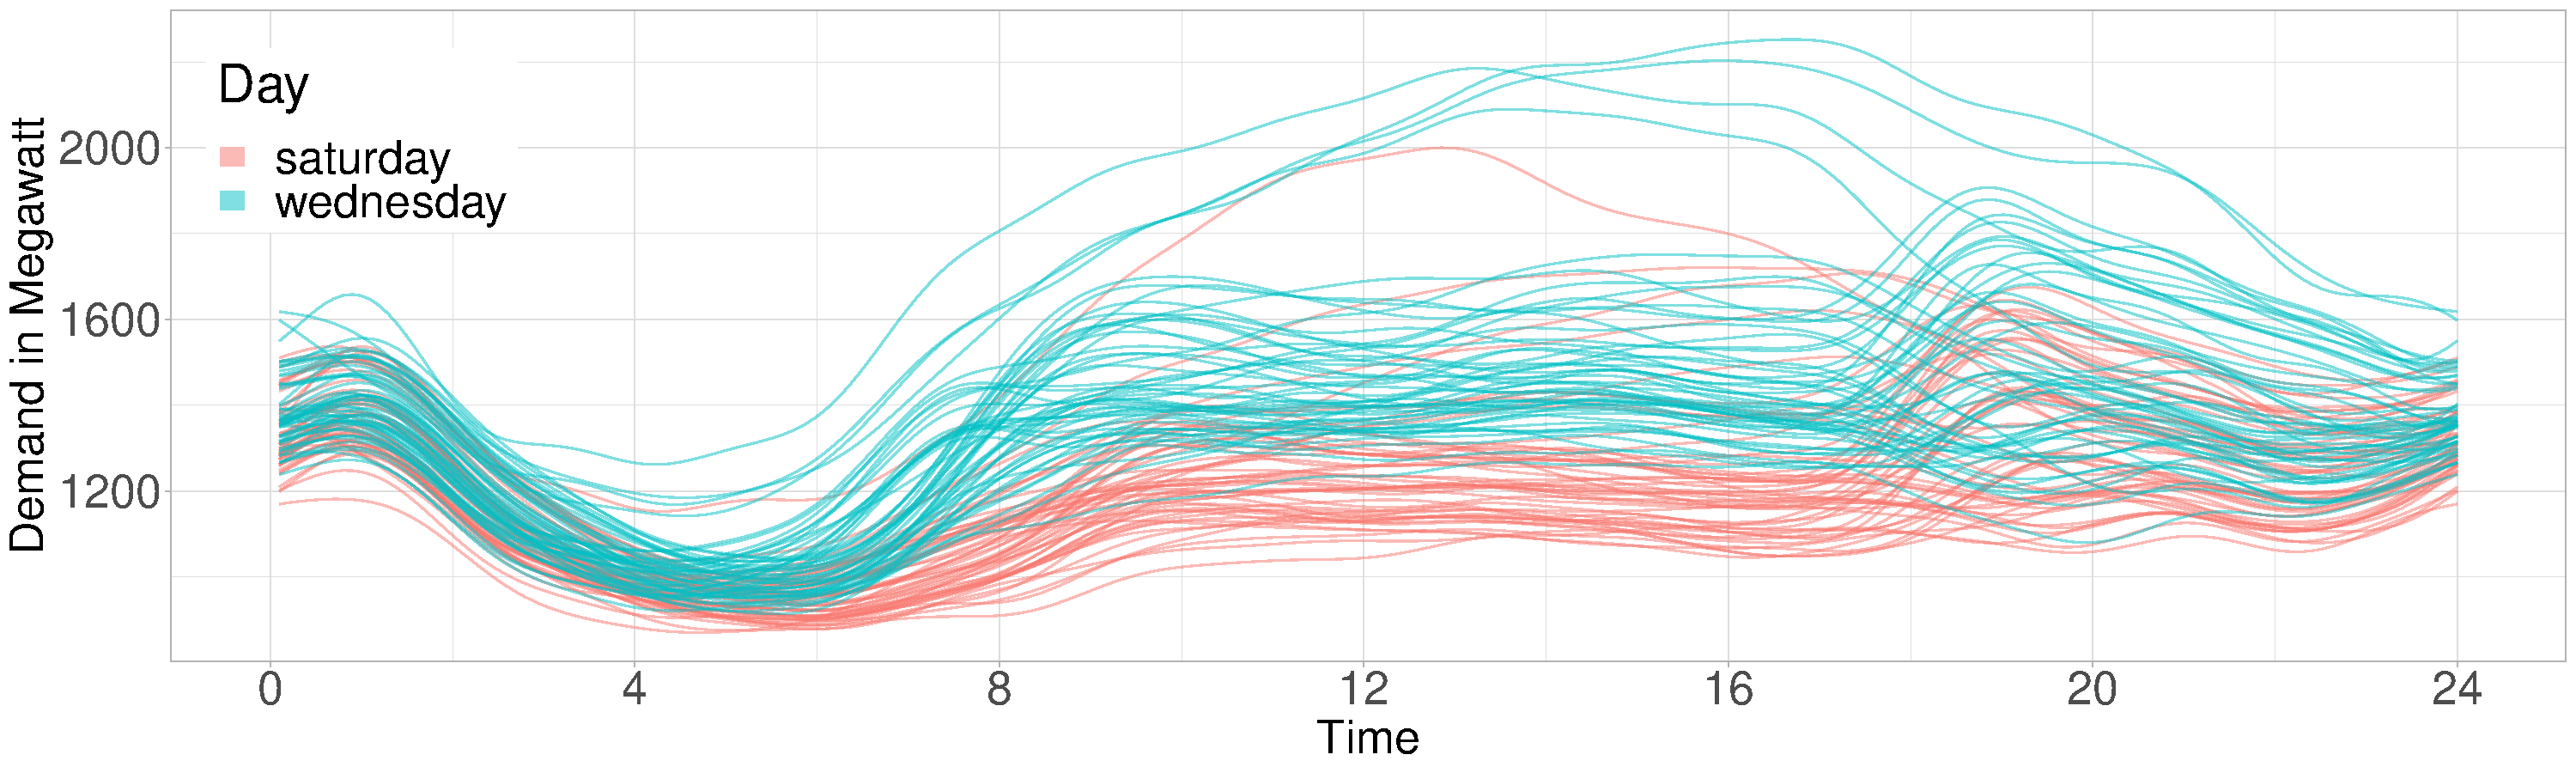
\includegraphics[width=1.1\textwidth]{../Graphics/electricity_demand_curves.PDF}
			}
			\caption{Electricity Demand in Adelaide}
			\label{electricity_demand}
		\end{figure}
	
		The question I want to study with the method presented in this thesis is whether electricity demand on working days and weekends can be seen as if they were generated by the same stochastic process. As this problem does not have the structure that an experiment as described in \cite{bugni_permutation_2021} possesses, a few problems have to be addressed before using the procedure. These adjustments are described below and some details are substantiated in Appendix \ref{Application_Appendix}.
	
		\subsection{Data Cleaning and Preprocessing}
			\subsubsection{Removal of Mondays and Fridays}
			One potential problem of this procedure is the question whether observations on different weekdays or days of the weekend can be seen as independent and identically distributed. While it seems reasonable to assume that demand may be similar on Saturdays and Sundays, it is questionable whether the same can be said for working days. 
			One potential problem is the ramping up and down of industrial production and commercial activity on Mondays and Fridays. Therefore, I decided to exclude these days from my analysis and only compare the weekend with Tuesdays, Wednesdays and Thursdays.
			
			\subsubsection{Holidays}
			Furthermore, holidays could appear more regularly on specific weekdays than others. Whereas on weekends, a holiday would not significantly influence the electricity demand due to the already reduced economic activity, this is different for weekdays. Therefore if holidays would occur systematically more often on specific days - such as for example Thursdays for the case of Germany - this could create problems. Therefore public holidays in Southern Australia, the Australian federal territory containing Adelaide, were excluded in the analysis. A list of holidays that were excluded is given in Appendix \ref{Application_Appendix}. Additionally, days immediately before and after holidays are excluded due to the same reason as Mondays and Fridays. This procedure of eliminating holidays from the data set removed 299 out of 3556 curves from the data set which was used in further steps of the analysis. \\
			
			\subsubsection{Detrending and Deseasoning}
			A third potential problem of this data set is its functional time series structure. For example, electricity demand might be systematically higher in the summer months due to the added energy consumption of air-conditioning units. Therefore, a simple interpretation of the data as generated by an i.i.d. process might be unsubstantiated and additional steps have to be made before the procedure can be justified. \\
			Additionally, it might be the case that electricity demand has a trend component that has to be removed before this method can reasonably be applied to this data. To combat this low frequency seasonal component due to the seasons and a potential long-term trend I specify a model as follows and demean the data as described below. For the estimation of this model, holidays and days immediately before and after holidays are excluded. Mondays and Fridays are included and removed from the data set after the estimation for the creation of the samples that are used to apply the method described in this thesis.
			\begin{equation}\label{Data_Cleaning}
				\begin{split}
					f_{\textit{demand}} = &f_{\textit{mean}} + f_{\textit{trend}}(\textit{year} - 1997) + \sum_{j = 2}^{12}\mathbbm{1}_{\left[\textit{month}\: = \: j\right]}f_{\textit{month}, j}\\
					 &+ \sum_{k = 2}^{7}\mathbbm{1}_{\left[\textit{day}\: = \: k\right]}f_{\textit{day}, k} + f_{\textit{random}}
				\end{split}	
			\end{equation}
			This is estimated with the usual theory for function-on-scalar regression which is described for example in \cite{ramsay_functional_2005}. Then, the following objects are used for the further treatment.
			\begin{equation}
				\tilde{f} = f_{\textit{mean}} + \sum_{k = 2}^{7}\mathbbm{1}_{\left[\textit{day}\: = \: k\right]}\hat{f}_{\textit{day}, k} + \hat{f}_{\textit{random}}
			\end{equation}
			The function-on-scalar regression described in Equation \ref{Data_Cleaning} was performed in R using the \textit{fda}\footcite{fda} package and gave the following results. As these are the results of a function-on-scalar regression, it is convenient to plot the resulting estimates as they are functions instead of giving the estimated Fourier coefficients.
			
			\begin{figure}[H]
				\makebox[\textwidth][c]{
				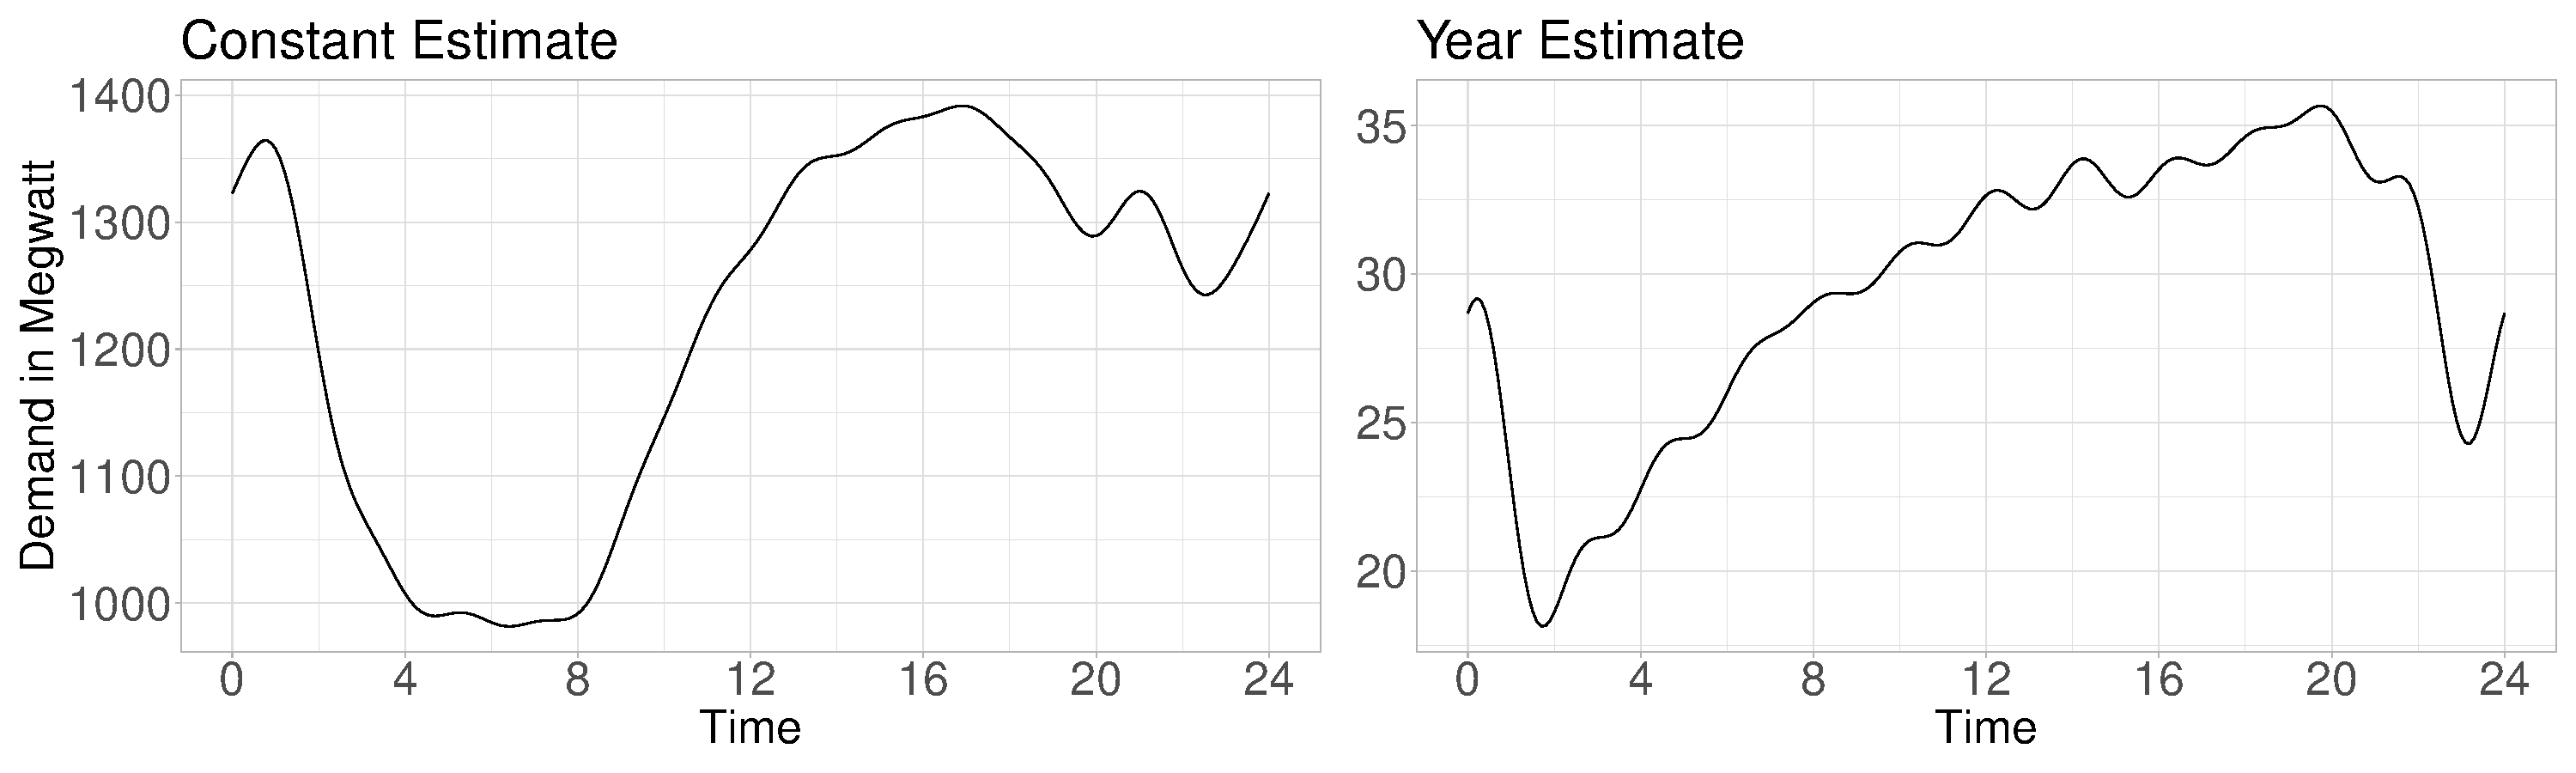
\includegraphics[width=1.1\textwidth]{../Graphics/estimate_const_year.PDF}
			}
				\caption{Estimates for the constant and year}
				\label{estimates_const_year}
			\end{figure}
		
			\begin{figure}[H]
				\makebox[\textwidth][c]{
				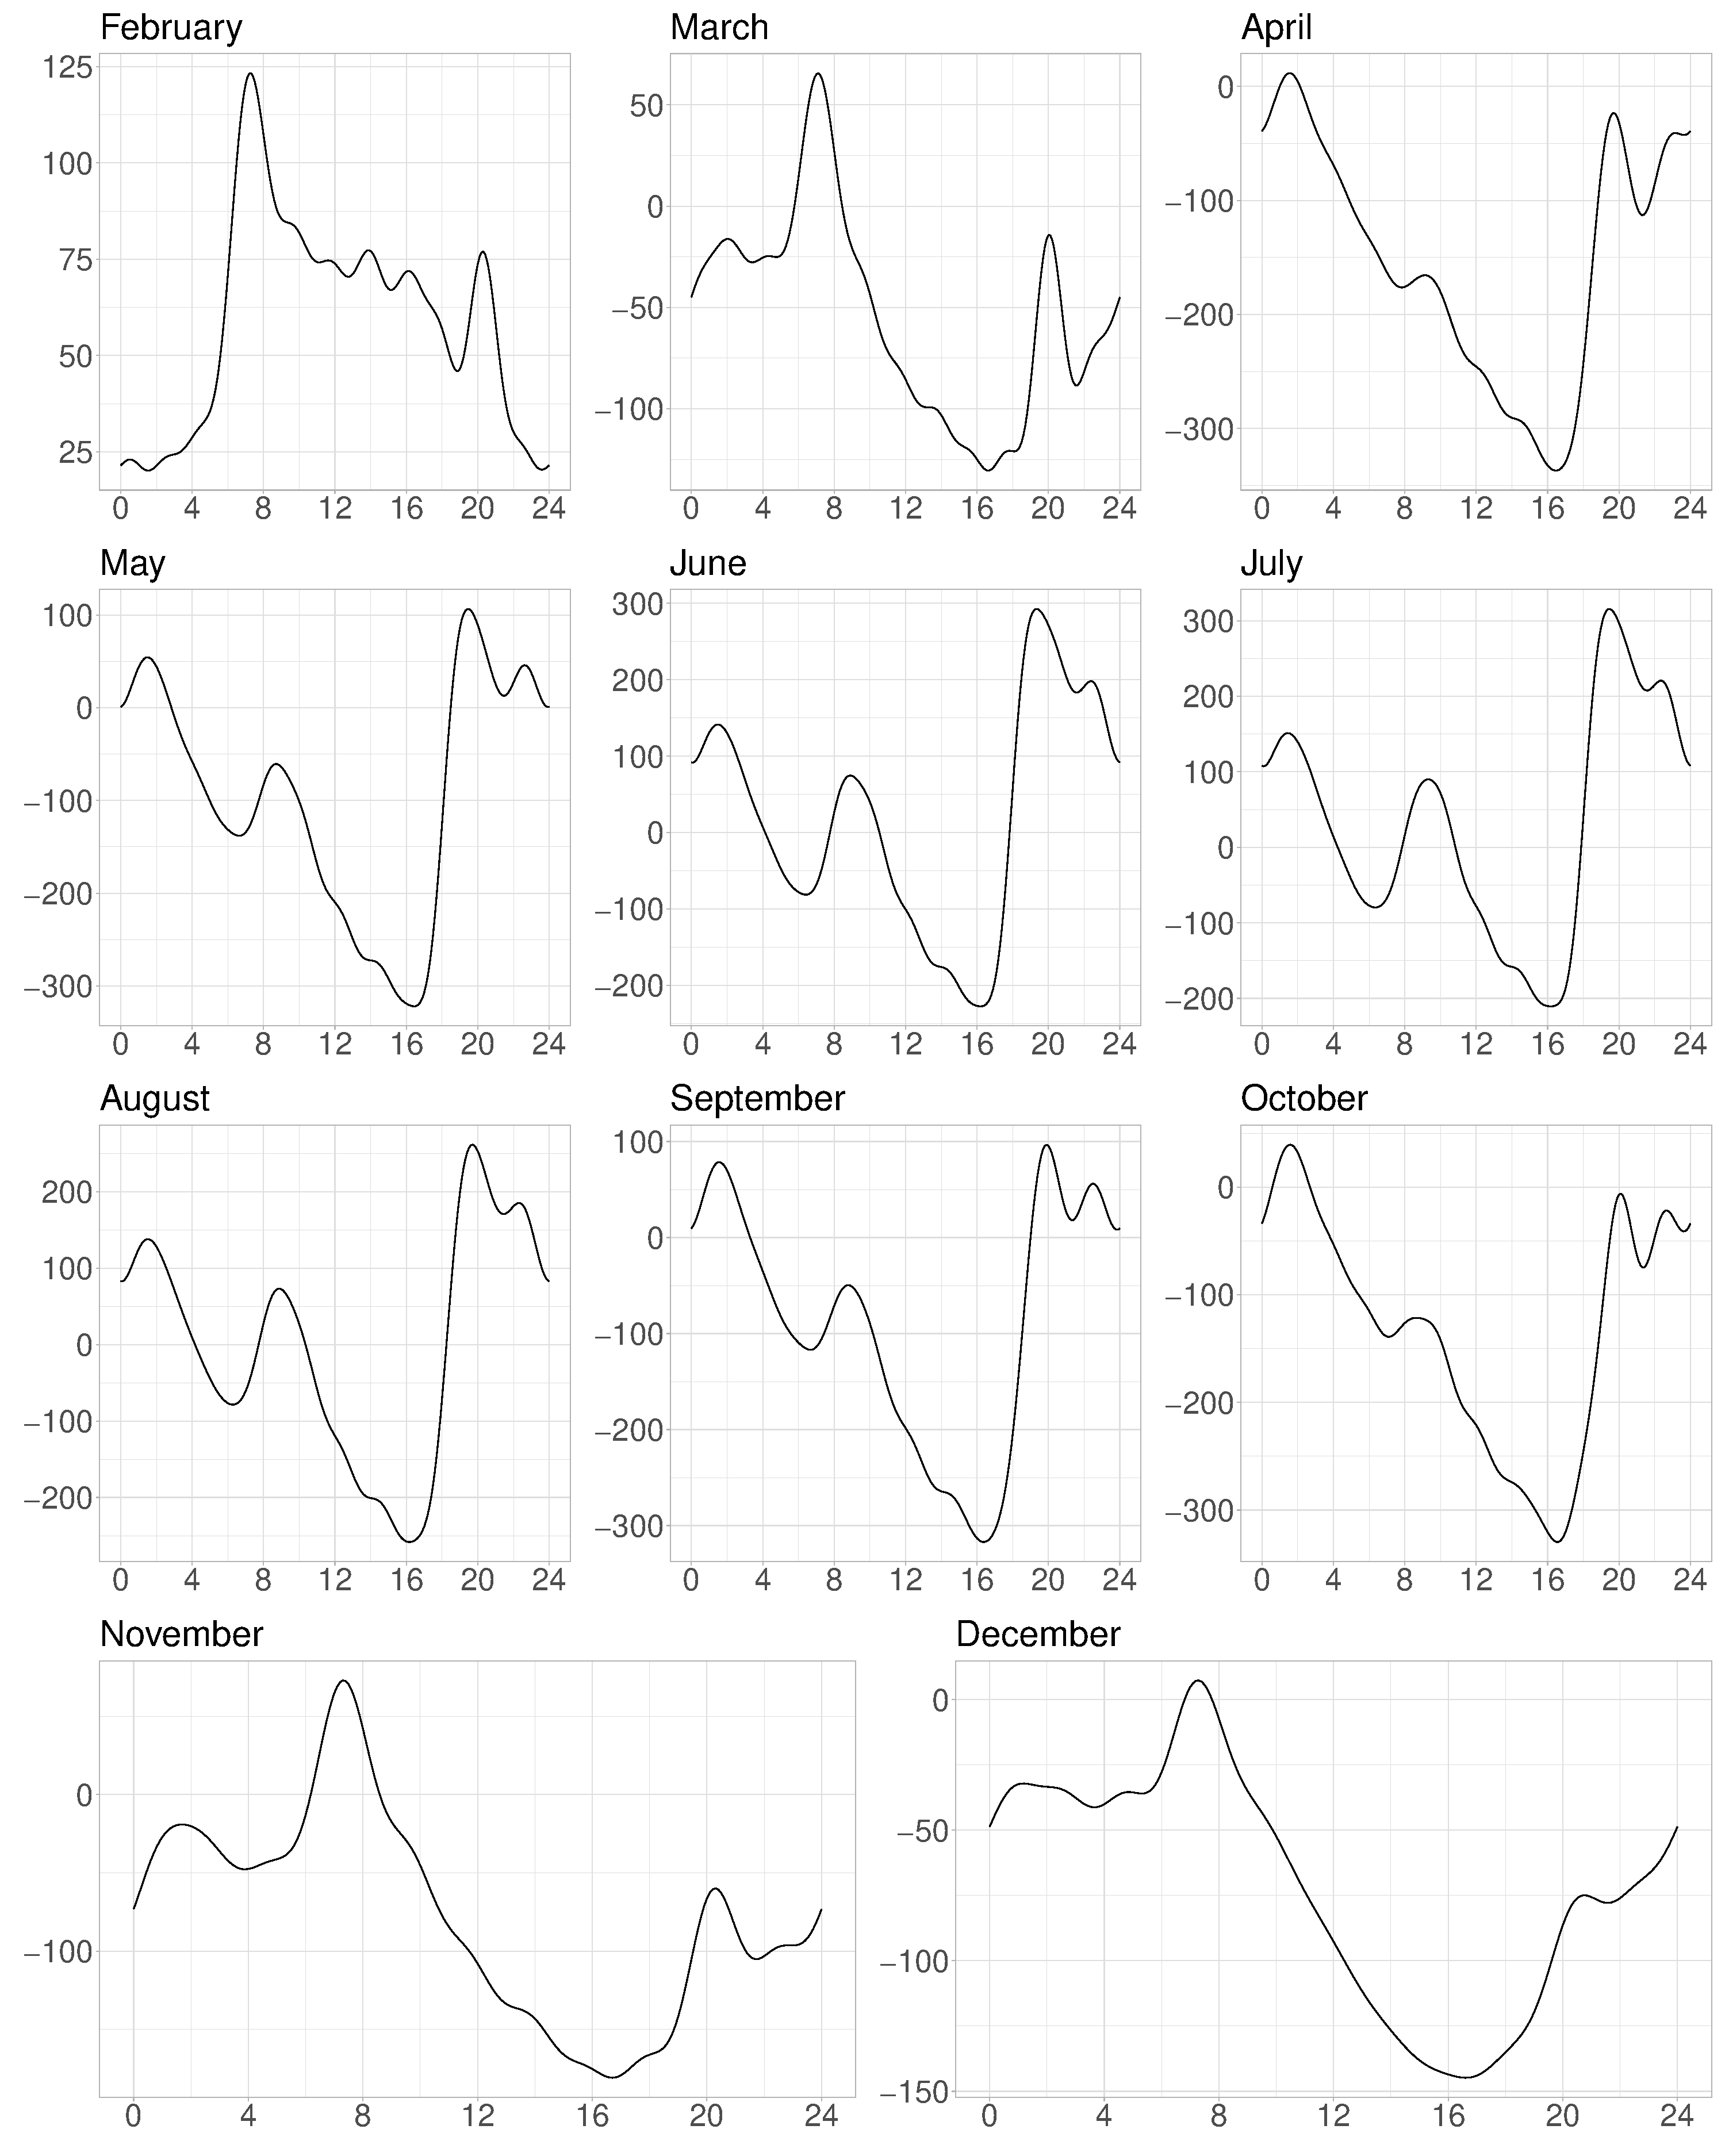
\includegraphics[width=1.1\textwidth]{../Graphics/estimate_months.PDF}
			}
				\caption{Estimates for the months (January as baseline)}
				\label{estimates_months}
			\end{figure}
		
			The estimated coefficient functions for the different weekdays are of special interest as they are directly linked to the problem that is to be studied using the method from \cite{bugni_permutation_2021}. In this case Sunday is the baseline and these curves describe the deviation relative to it.
			\begin{figure}[H]
				\makebox[\textwidth][c]{
				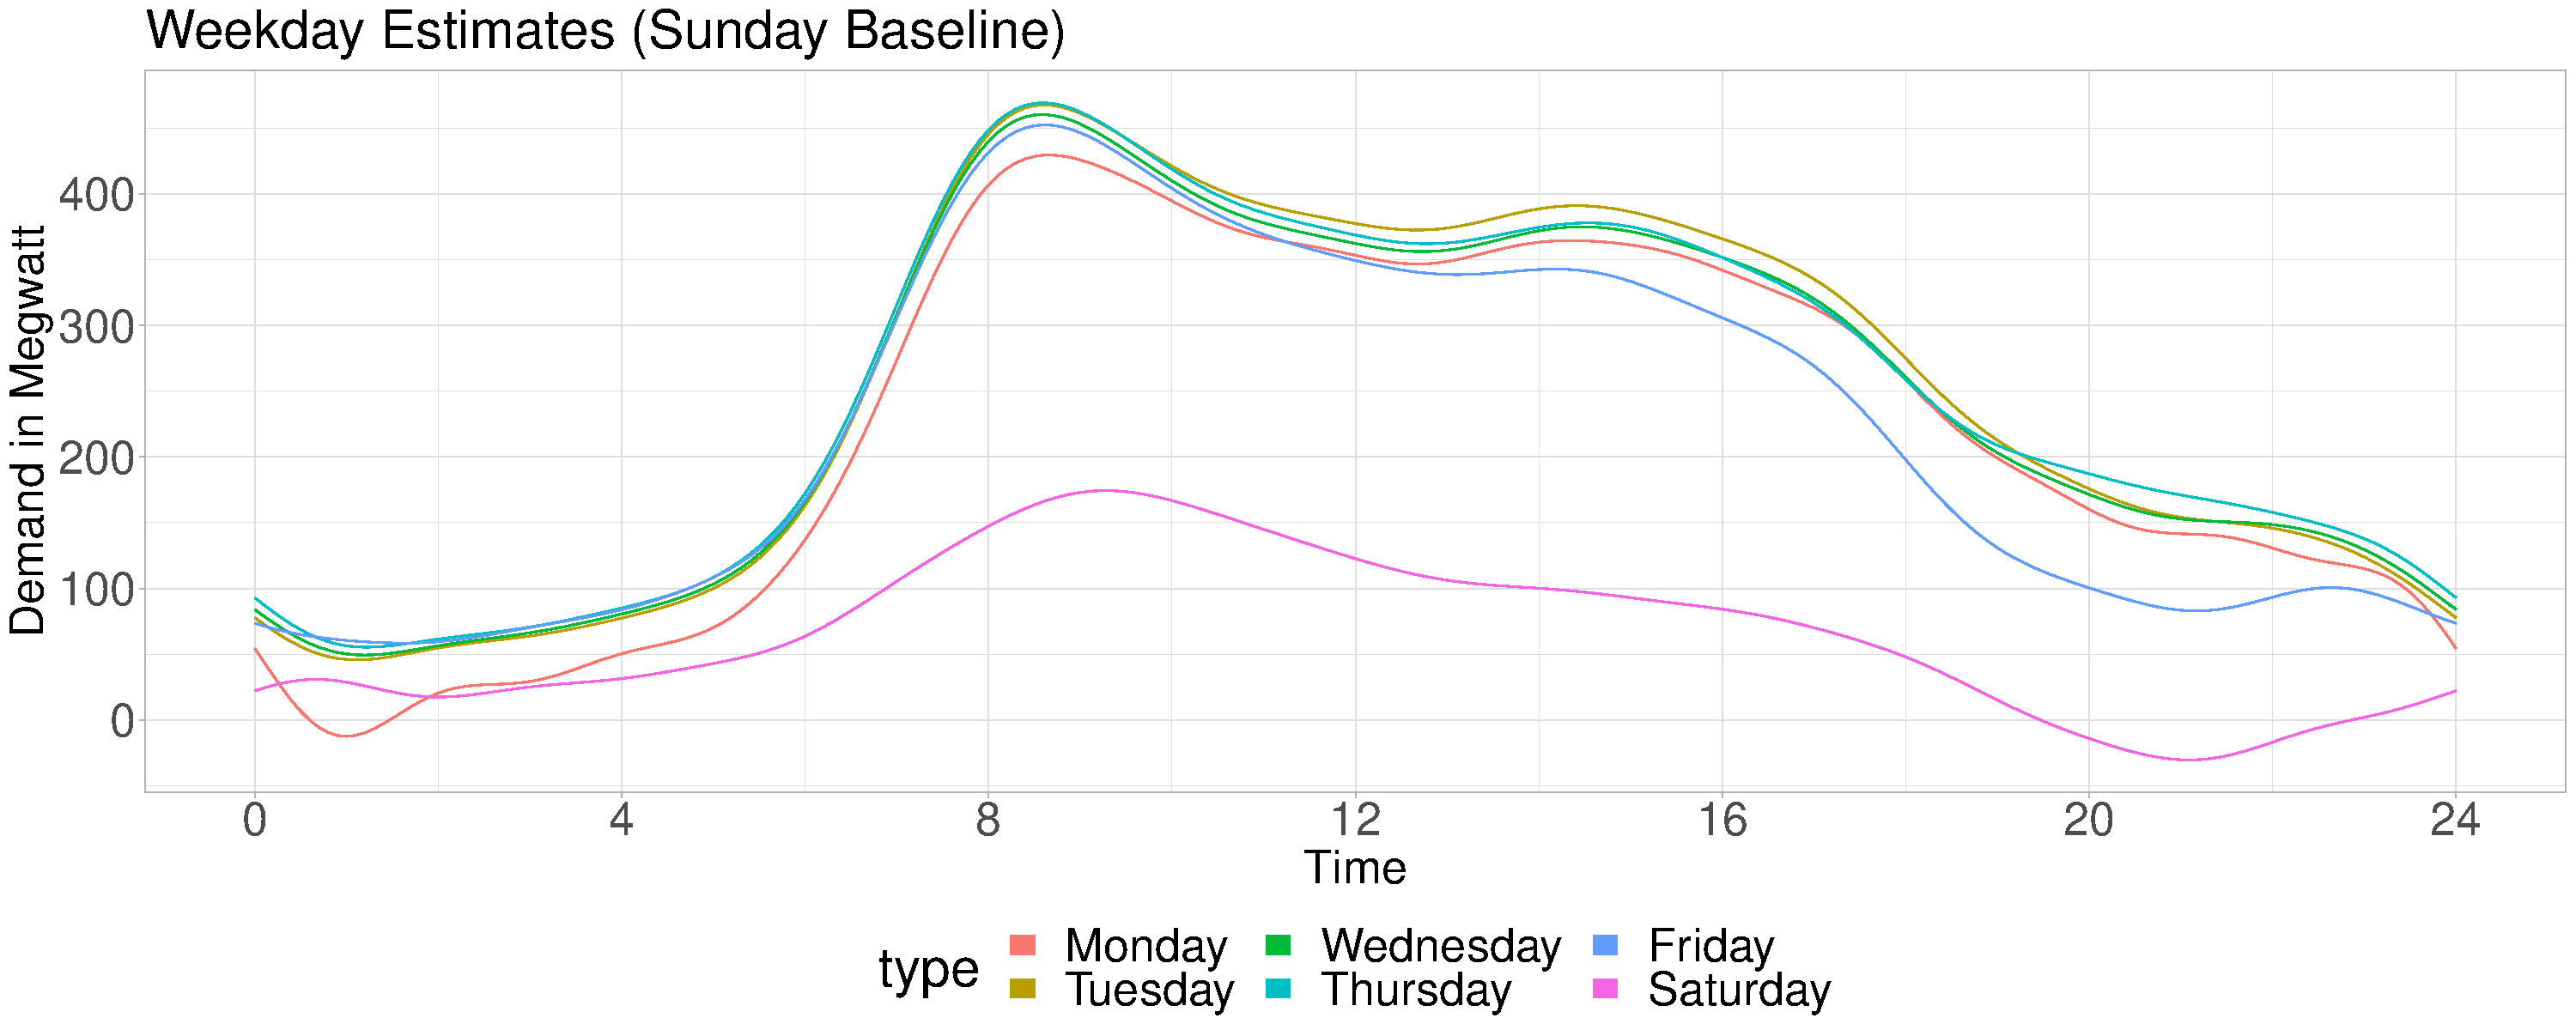
\includegraphics[width=1.1\textwidth]{../Graphics/estimate_weekdays.PDF}
			}
				\caption{Estimates for the weekdays (Sunday as baseline)}
				\label{estimates_weekdays}
			\end{figure}
			This diagram already hints at a considerable mean shift between the working days and the weekend. As these estimates also hint at a considerable difference between Saturdays and Sundays, it could be advisable to treat them as non-identically distributed. Therefore, a comparison between Saturdays on the one hand and Tuesdays, Wednesdays and Thursdays on the other might be better suited for the test procedure.
			
		\subsection{Test from \cite{bugni_permutation_2021}}
			After cleaning the data as described in the previous section, we can now apply the method from \cite{bugni_permutation_2021}.
			To give a visualization of what these cleaned curves look like, Figure \ref{electricity_demand_cleaned} shows randomly chosen curves observed on Wednesdays and Saturdays that were prepared with the procedure described above.
			
			\begin{figure}[H]
				\makebox[\textwidth][c]{
				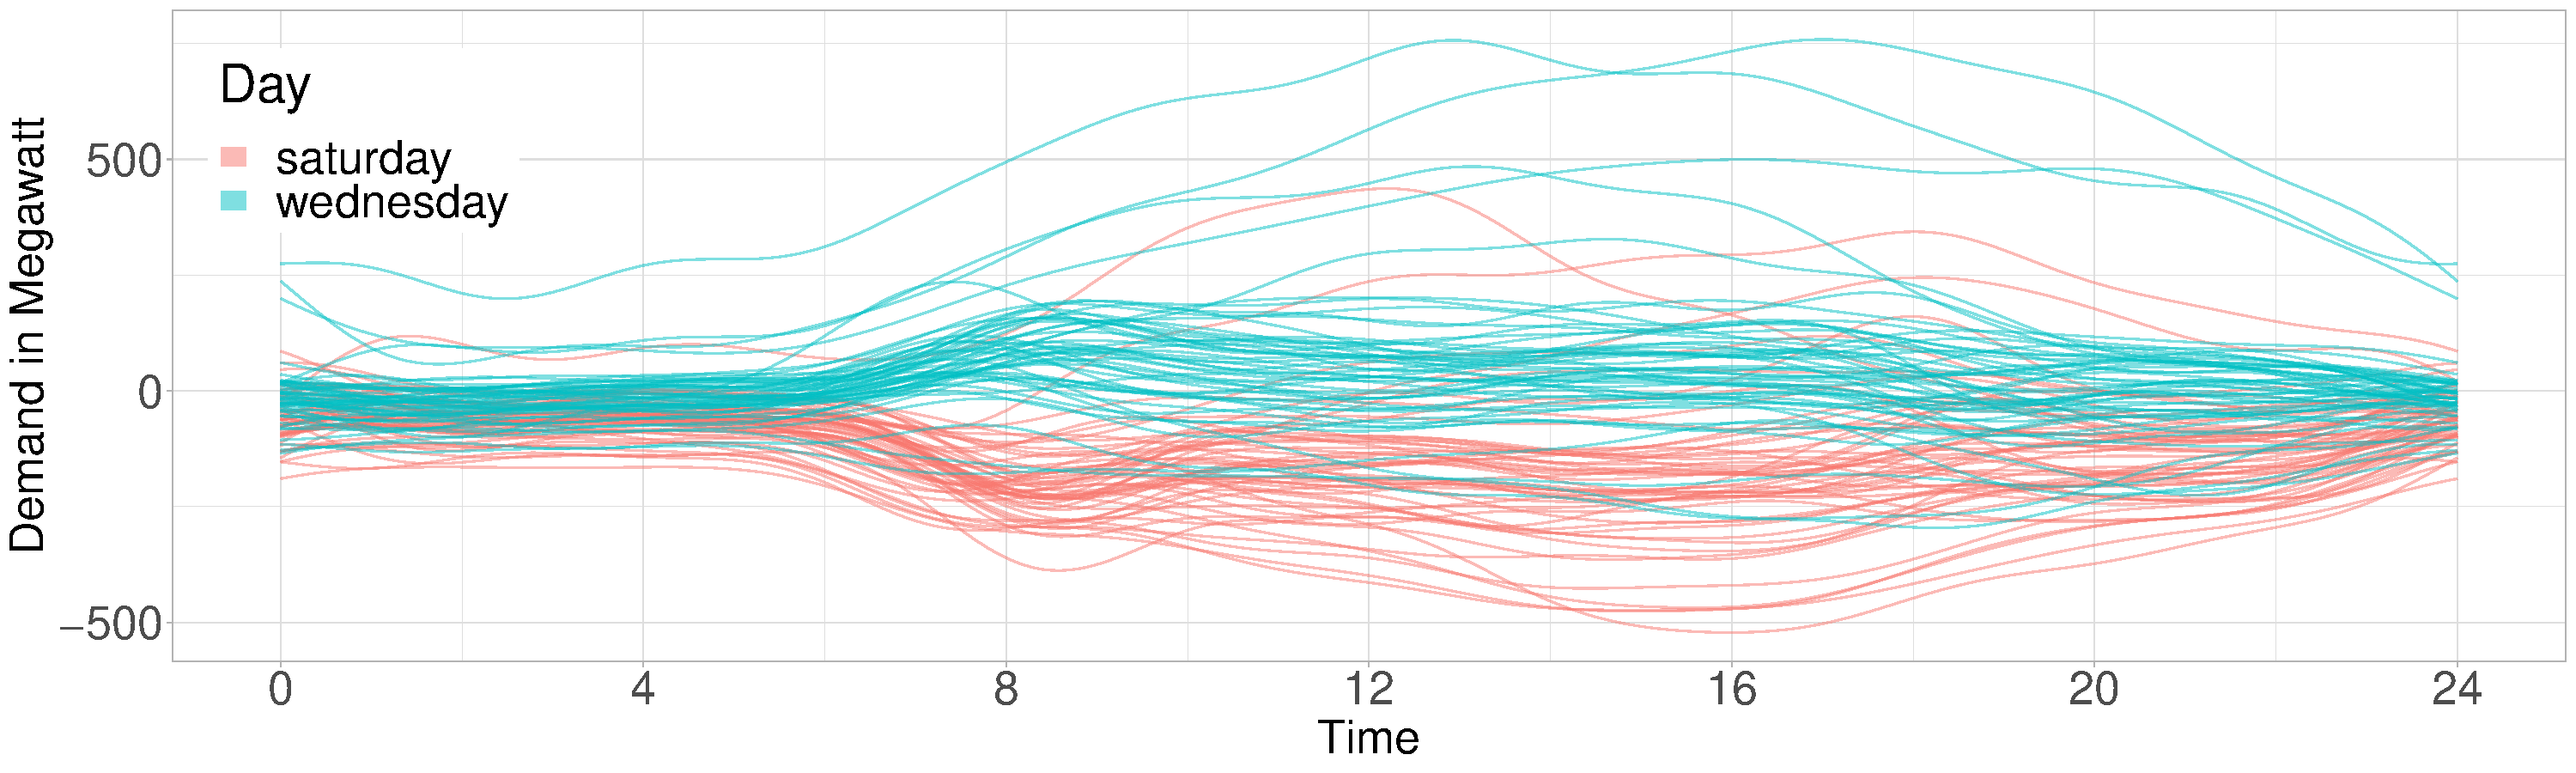
\includegraphics[width=1.1\textwidth]{../Graphics/electricity_demand_curves_cleaned.PDF}
			}
				\caption{Pre-Processed Electricity Demand in Adelaide}
				\label{electricity_demand_cleaned}
			\end{figure}
	
	\section{Outlook}\label{Outlook}
		After studying the method developed by \cite{bugni_permutation_2021} in detail there are a few points that might be interesting for further research. In the following I name a few that could be very interesting extension to this thesis.
		
		\paragraph{Simulations for Different Measures}
		
		\paragraph{Simulations comparing choices of $w(t)$ and  $\left(\rho_i\right)_{i = 1, \dots, K}$}
		
		\paragraph{Simulation Settings where the Distribution of Fourier Coefficients is changed}
			\begin{itemize}
				\item Use dgp similar to the way we construct the measure (draw fourier coefficients from some distribution)
				\item Same mean for fourier coefficients, but different distribution of error terms
			\end{itemize}
		
		\paragraph{Simulations for Unbalanced Sample Sizes}
		
		\paragraph{Application that has a more complex difference structure}
			\begin{itemize}
				\item Audio-Curves
				\item Movement-Curves
			\end{itemize}
		
		
	
	\newpage
	\section{Bibliography}
	\printbibliography[heading=none]
	
	\newpage
	\cleardoublepage
	\pagenumbering{roman}
	\setcounter{page}{1}
	\section{Appendix}
	
		\subsection{Multiple Testing}\label{Multiple_Testing}
			When testing statistical hypotheses, it is often helpful or even necessary to test multiple hypotheses independently of each other. One setting where this could be useful is when we want to combine the desirable properties of two tests, as is done by \cite{bugni_permutation_2021}. If the tests do not perfectly depend on each other, this creates a problem relating to the size of the combined test.
			
			\begin{definition}[Family-wise Error Rate]
				The family-wise error rate is the probability of making at least one type-1 error when performing multiple hypothesis tests.
			\end{definition}
		
				The most straightforward correction for this multiple testing problem is the so-called Bonferroni Correction. Introduced by \cite{dunn_multiple_1961}, it is based on Boole's Inequality, which is sometimes referred to as the Bonferroni Inequality.
				\begin{equation}
						\mathbb{P}\left[\bigcup_{i = 1}^{\infty} A_i\right] \leq \sum_{i = 1}^{\infty} \mathbb{P}\left[A_i\right]
					\end{equation}
				for a countable set of events $A_1, A_2, \dots$.
		
		\subsection{Derivation of Asymptotic Distribution}\label{asymp_deriv}
			Here I will derive the asymptotic distribution
			
		\subsection{Application Data Cleaning}\label{Application_Appendix}
			\subsubsection{Excluded Holidays}
			Holidays that were excluded in the analysis are the following\footnote{These were taken from \url{https://www.australia.gov.au/public-holidays} accessed on 20.05.2022.}: New Year's Day, Australia Day, March Public Holiday, Good Friday, Holy Saturday, Easter Monday, Anzac Day, Queen's Birthday, Labour Day, Christmas Day, Christmas Eve, Christmas Day, Proclamation Day and New Year's Eve. Sunday is nominally a public holiday in South Australia. Easter Sunday is therefore not a special public holiday, but due to its prominence it was excluded in this analysis.
			
			As Australia replaces some holidays that fall on weekends with substitute holidays on the next working day, these were also excluded. For the South Australia, this can occur for New Year's Day, Australia Day, ANZAC Day, Christmas Day, Proclamation Day and New Year's Eve.
		
			\subsubsection{Detrending and Deseasoning Results}
			
			
			
	\newpage
	\thispagestyle{empty}
	\section*{Versicherung an Eides statt}	
	
		\vspace{3cm}
		
		Ich versichere hiermit, dass ich die vorstehende Masterarbeit
		selbstständig verfasst und keine anderen als die angegebenen Quellen
		und Hilfsmittel benutzt habe, dass die vorgelegte Arbeit noch an keiner
		anderen Hochschule zur Prüfung vorgelegt wurde und dass sie weder
		ganz noch in Teilen bereits veröffentlicht wurde. Wörtliche Zitate und
		Stellen, die anderen Werken dem Sinn nach entnommen sind, habe ich
		in jedem einzelnen Fall kenntlich gemacht.
		
		\vspace{2cm}
		Bonn, XX.07.2021 \hrulefill \\
		\hspace*{0mm}Jakob R. Juergens
		
		\vspace{\fill}
\end{document}